% \documentclass[10pt,handout,usenames,dvipsnames,pdf]{beamer}
\documentclass[10pt,usenames,dvipsnames,pdf]{beamer}

\usepackage[portuguese,english]{babel}
\usepackage[backend=biber,style=authoryear-icomp,natbib=true,url=false,doi=true]{biblatex}

\usepackage[notesposition=right,duration=20,lastminutes=5]{pdfpc}
\usepackage{appendixnumberbeamer}

\usepackage[scale=2]{ccicons}

\usepackage{hyperref}
\usepackage{booktabs}
\usepackage{multirow}
\usepackage{bookmark}

\usepackage{graphicx}
\usepackage{csquotes}
\usepackage{float}

% Bibliography
% \addbibresource{../references.bib}

% PDF Presenter Console (pdfpc) Notes
\setbeamertemplate{note page}{\pagecolor{black!2}\normalsize\insertnote}

% \setbeameroption{hide notes}
\setbeameroption{show notes on second screen=right}

\newcommand<>{\talknote}[1]{\only#2{\note[item]{\textbf{#1}}\relax}}

% PDF Metadata
\hypersetup{
 pdftitle = {Docker Workshop},
 pdfauthor = {Pedro Rodrigues},
 pdfsubject = {Docker},
 pdfkeywords = {Docker, Workshop, NEI},
 pdfproducer = {Latex Beamer with hyperref},
 pdfcreator = {lualatex},
}

% Beamer Theme
\usetheme[progressbar=frametitle, background=light]{metropolis}
\metroset{block=fill}

% Title Page Settings
\title{Docker Workshop}
\author{Pedro Rodrigues} 

\date{\footnotesize April 12, 2023}
\institute{University of Coimbra \\ Department of Informatics Engineering}
\titlegraphic{\vspace{4cm}\hspace{7cm}
\includegraphics[keepaspecratio,width=2.5cm]{./assets/docker.png}} 

\begin{document}

\begin{frame}[noframenumbering, plain]
	\titlepage
  \talknote{Boa Tarde!}
  \talknote{Mostrar QR Code Certificado}
\end{frame}

\begin{frame}[noframenumbering, plain]
	\centering
	\emph{\textbf{\Large{Certificado de Participação}}}
	\begin{figure}
		
\includegraphics[scale=0.3]{./assets/certificate.pdf}
	\end{figure}
	\emph{\textbf{\Large{Workshop de Docker}}}
  \talknote{Perguntar se alguém teve problemas a instalar o software}
\end{frame}

\begin{frame}{What is Docker?}
	\begin{center}
		\emph{\large{\textbf{``Docker is an open platform for developing, shipping, and running applications''}}}
	\end{center}
	\begin{itemize}
		\item \alert{Separates} your applications from your infrastructure.
		\item \alert{Manages} your infrastructure in the same way you manage your applications.
		\item \alert{Reduces} the delay between writing code and running it in production.
	\end{itemize}
  \talknote{Quem desenvolve a aplicação não precisa de se preocupar com a configuração/manutenção da infrastrutura}
  \talknote{As aplicações são geralmente configuradas usando ficheiros, com o docker podemos definir a infrastrutura onde aplicação vai correr da mesma forma}
  \talknote{Otimiza a pipeline de desenvolvimento visto que reduz o esforço do deploy e manutenção e testing de uma forma geral}

\end{frame}

\begin{frame}{Why use Docker?}
	\begin{figure}
		
\includegraphics[scale=0.3]{./assets/meme.jpg}
	\end{figure}
  \talknote{Quem é que nunca teve problemas com isto?}
	\talknote{
    Possiveis Problemas
		\begin{itemize}
			\item Ficheiros em falta
			\item Versão software, software não existe para o sistema operativo
			\item Configurações diferentes em cada máquina
      \item Ou simplemente não nos apetece instalar o software na nossa maquina...
		\end{itemize}
	}
  \talknote{Facilita imenso a vida de quem desenvolve software e de quem dá deploy (pode ser a mesma pessoa)}
\end{frame}

\begin{frame}{Containers and Virtual Machines}
	\begin{figure}
		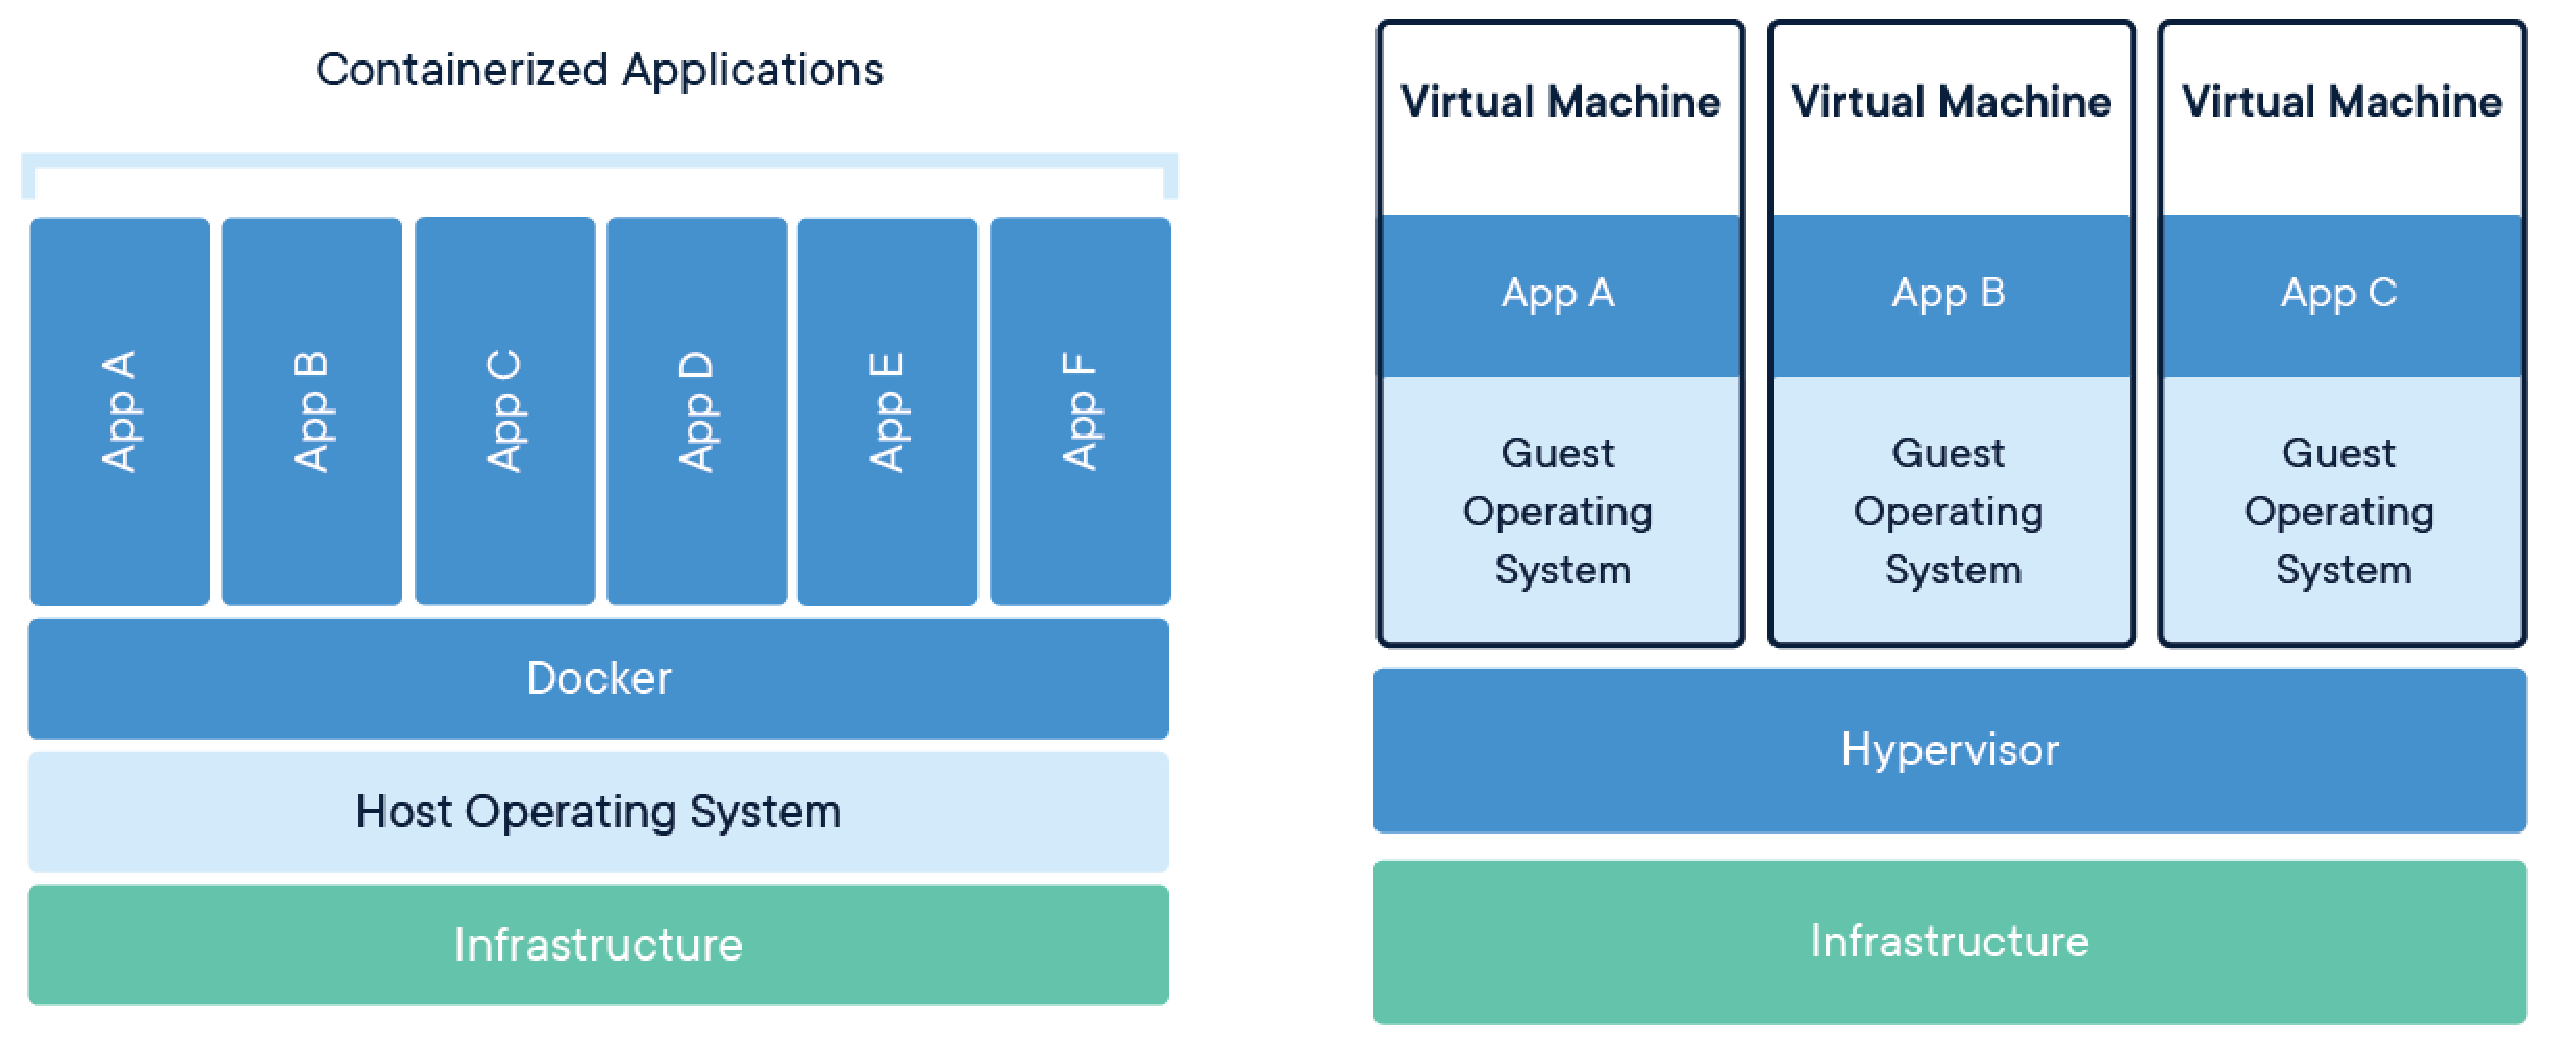
\includegraphics[scale=0.25]{./assets/vm-container.pdf}
	\end{figure}
  \talknote{Containers são ambientes isolados onde aplicações correm}
  \talknote{Uma VM é uma abstração do hardware fisico (hypervisor)}
  \talknote{Uma VM precisa de um sistema operativo (guest), é lenta, e necessita de bastantes recursos}
  \talknote{Containers são processos que correm num namespace isolado (linux feature)}
  \talknote{Containers permitem correr varios processos, são leves, usam o sistema operativo atual, são rapidas e precisam de menos recursos de hardware}
\end{frame}

\begin{frame}{Architecture Overview}
	\begin{figure}
		\centering
		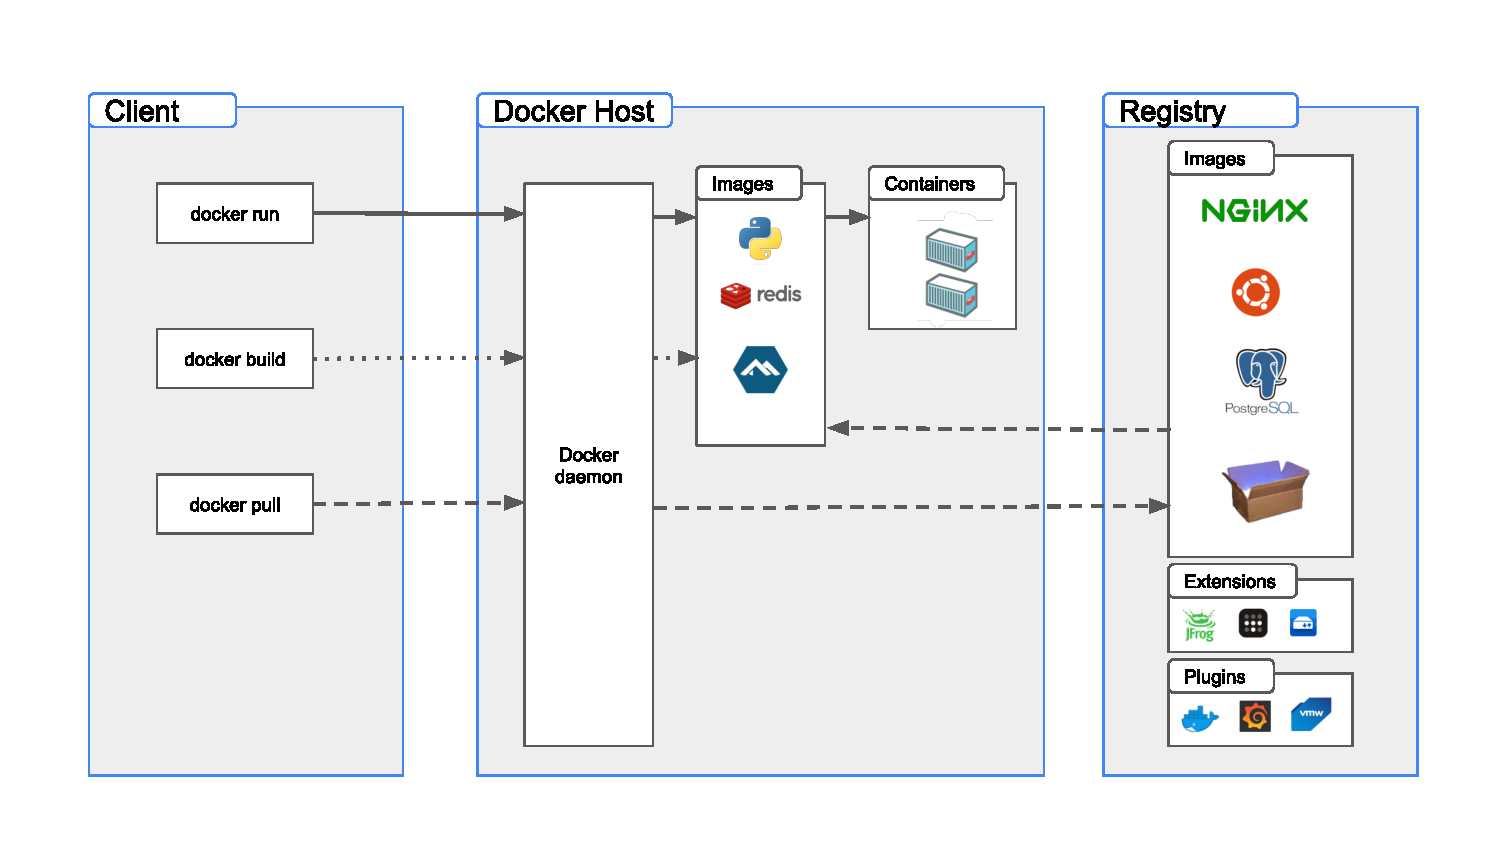
\includegraphics[scale=0.4]{./assets/architecture.pdf}
	\end{figure}
  \talknote{Arquitetura Cliente Servidor (engine/dockerd)}
  \talknote{Existe o podman que é similar ao docker mas é daemonless}
  \talknote{Cliente (Desktop, CLI, etc..) liga-se ao Server (Docker Engine) através de uma unix socket REST API (por ser mais mais rapido) ``curl --unix-socket /var/run/docker.socket http://localhost/version''}
  \talknote{Registo (Remote) onde se podem fazer download de imagens, plugins e extensões}
  \talknote{Docker Hub é um registo aberto}
\end{frame}

\begin{frame}{Operating System Support}
	\begin{center}
		\emph{\textbf{Docker runs on all major operating systems!}}
		\begin{figure}
			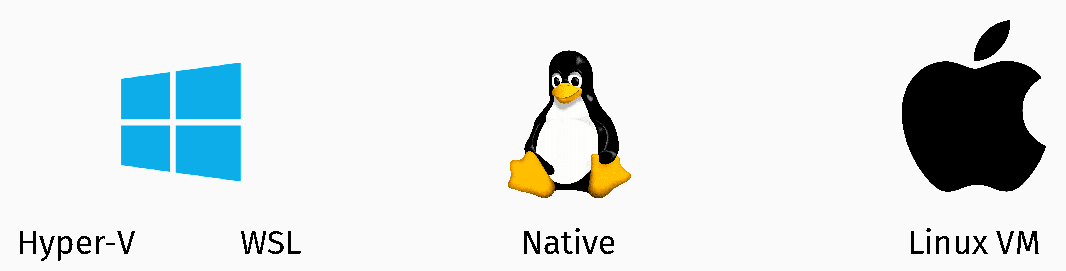
\includegraphics[scale=0.4]{./assets/os.pdf}
		\end{figure}
	\end{center}
\end{frame}


\begin{frame}{Images and Containers}
	\begin{figure}
		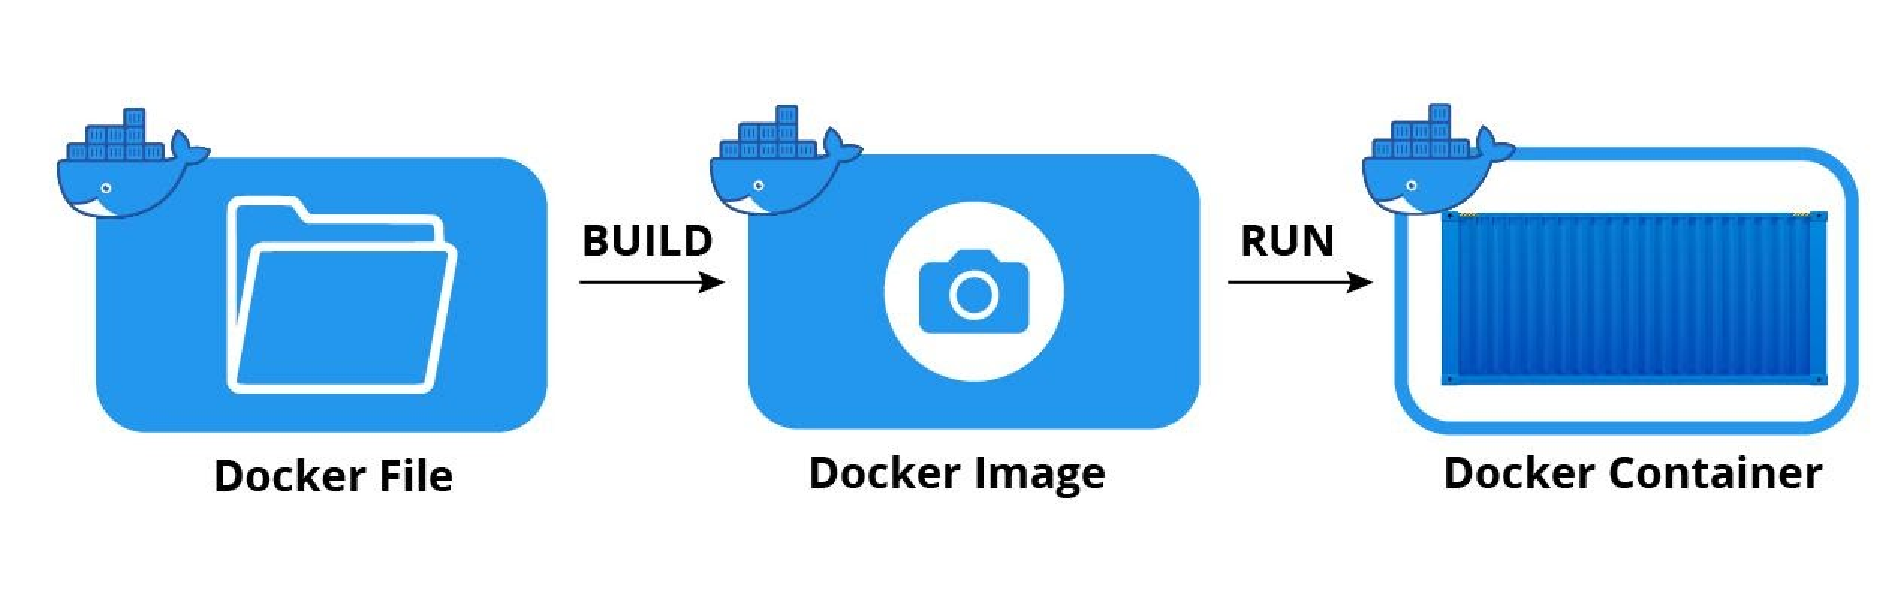
\includegraphics[scale=0.3]{./assets/pipeline.pdf}
	\end{figure}
\end{frame}

\begin{frame}[standout]
	Let's get to work?
  \talknote{Começar por trabalhar um bocado com o docker client (CLI).}
  \talknote{Trabalhar com imagens e containers.}
  \talknote{Criar a nossa propria imagem com um dockerfile.}
  \talknote{Mostrar o docker compose.}
  \talknote{Cenas interessantes que se pode fazer com docker.}
  \talknote{Coisas avançadas: Multi-Stage Builds, Networks, Volumes.}
  \talknote{Referir tecnologias como jenkins, kubernetes e cenas interessantes para quem quer ir mais in depth como o ``bocker''.}
\end{frame}

\end{document}

